%!TEX root = syntheyes15.tex

\section{Rendering photo-realistic training images}

% define each rendered image by c, g, L
Once our eye-region model is prepared, we render it from a wide range of camera positions and lighting conditions.

We briefly describe how we use image-based lighting \cite{debevec2002image} to model a wide range of realistic lighting conditions, and finally discuss the details of our rendering setup.

For a chosen eye-region model configuration, each rendered image is determined by parameters $(\mathbf{c}, \mathbf{g}, L)$ -- 3D camera position $\mathbf{c}$; 3D gaze vector $\mathbf{g}$; and lighting environment $L$. As shown in \autoref{fig:cam_pos}, $\mathbf{c}$ is chosen by iterating over spherical coordinates $(r, \theta, \phi)$, centered around the eyeball center. Images are rendered with an orthgraphic camera, as this simulates an eye region-of-interest being cropped from a wide-angle camera image, so we set $r\!=\!1$ for convenience. At each camera position $\mathbf{c}$, we render multiple images with different gaze vectors to simulate the eye looking in different directions. Examples with fixed $L$ are shown in \autoref{fig:cam_pos_example_renders}. Gaze vectors $\mathbf{g}$ are chosen by first pointing the eye directly at the camera (simulating eye-contact), and then modifying the eyeball's pitch ($\alpha$) and yaw ($\beta$) angles over a chosen range.

A consequence of this approach is the possibility of rendering ``unhelpful'' images that either simulate impossible scenarios (e.g. an eyeball rotated beyond its anatomical limit), or are not useful for training (e.g. eyes rolled back so none of the iris is visible). To avoid violating anatomical constraints, we only render images for valid eyeball rotations $|\alpha|\!\leq\!25^{\circ}$ and $|\beta|\!\leq\!35^{\circ}$ \cite{MIL-STD-1472G}. Before rendering, we also verify that the projected 2D pupil center in the image will be within the 2D polygon of the eyelid landmarks using a point-in-polygon algorithm -- this avoid us rendering images where too little of the iris is visible.

\begin{figure}
    \centering
    \begin{subfigure}[t]{0.48\columnwidth}
        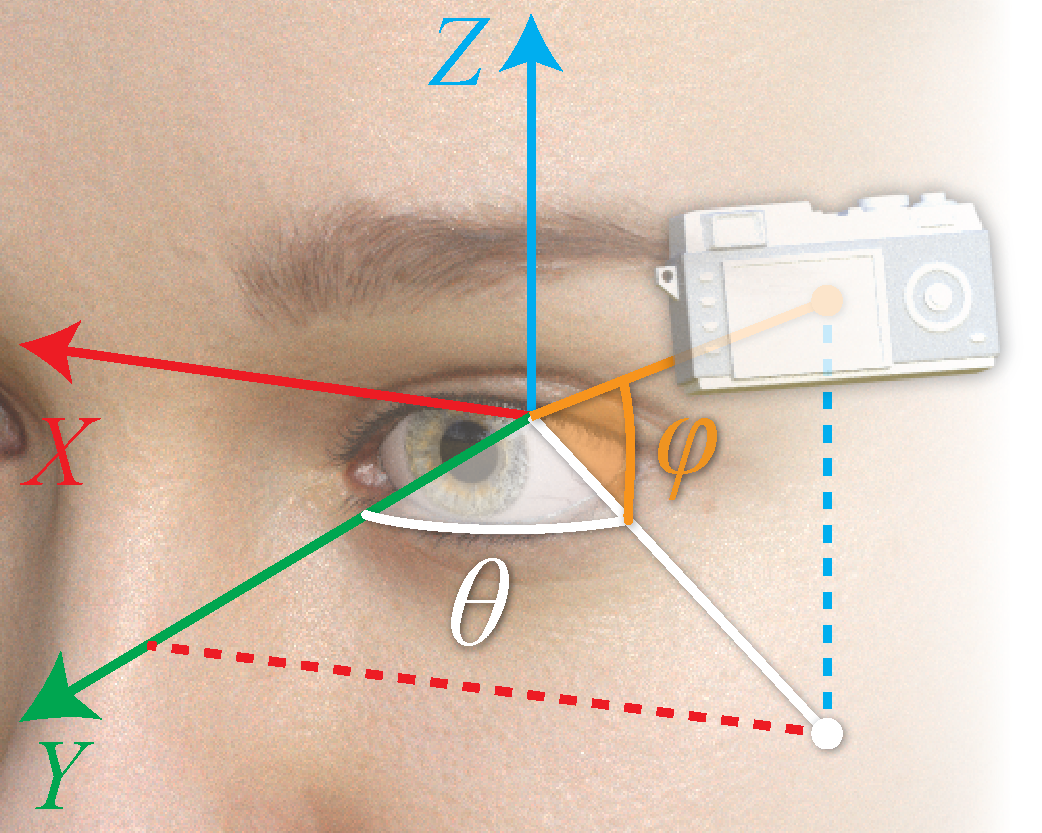
\includegraphics[width=\textwidth]{camera_position}
        \caption{The camera is positioned using spherical coordinates}
        \label{fig:cam_pos_spher_coords}
    \end{subfigure}
    \hfill
    \begin{subfigure}[t]{0.48\columnwidth}
        \includegraphics[width=\textwidth]{camera_pos_sample_renders_7x7}
        \caption{Example renderings from one camera position}
        \label{fig:cam_pos_example_renders}
    \end{subfigure}
    \caption{\ref{fig:cam_pos_spher_coords} shows how we position the camera to simulate changes in head pose. At each camera position, we render many eye images (\ref{fig:cam_pos_example_renders}) by posing the eyeball model.}
    \label{fig:cam_pos}
\end{figure}

\subsection{Lighting}

One of the main challenges in eye tracking is illumination invariance -- a good system should be able to track gaze under a range of real-life lighting conditions. One way of achieving this is using a training set that covers 

\begin{figure}
    \includegraphics[width=0.24\columnwidth]{fig_env_1} \hfill
    \includegraphics[width=0.24\columnwidth]{fig_env_2} \hfill
    \includegraphics[width=0.24\columnwidth]{fig_env_3} \hfill
    \includegraphics[width=0.24\columnwidth]{fig_env_4}
    \caption{Appearance variation from lighting is modelled with poseable high-dynamic-range environment maps \cite{debevec2002image}.}
    \label{fig:participants}
\end{figure}

\subsection{Computational setup}

We can rapidly generate diverse datasets much faster than manual collection and annotation.